\documentclass[tikz,border=10pt,12pt]{standalone}
% Shared preamble for standalone-compiled dc_paper figures.
% Copies just the bits of dc_paper.tex's preamble that figures need.

\usepackage{amsmath,amssymb,amsthm,mathtools,bm}
\usepackage{siunitx}
\sisetup{detect-all,group-separator={,},per-mode=symbol}

\usepackage[T1]{fontenc}
\usepackage{xcolor}
\usepackage{enumitem}
\usepackage{mathpazo}                % Palatino body + matching math
\usepackage[scaled=0.92]{helvet}     % Helvetica sans
\usepackage{courier}                 % monospace
\usepackage{microtype}

% --- IA brand colour palette (must match dc_paper.tex) ---
\definecolor{iadark}{HTML}{1B1815}
\definecolor{iabone}{HTML}{FAFAF7}
\definecolor{iaaccent}{HTML}{A04A1F}
\definecolor{iataupe}{HTML}{F2EDE6}
\definecolor{iarule}{HTML}{3A332D}
\definecolor{iagrey}{HTML}{5A524A}

% --- graphics ---
\usepackage{tikz}
\usepackage{circuitikz}
\usepackage{pgfplots}
\pgfplotsset{compat=1.18}
\usetikzlibrary{arrows.meta,positioning,shapes.geometric,calc,fit,
                decorations.pathreplacing,decorations.markings,
                shadows.blur,backgrounds}

% --- math macros from dc_paper.tex preamble (figures use them) ---
\newcommand{\E}{\mathbb{E}}
\newcommand{\Var}{\operatorname{Var}}
\newcommand{\Cov}{\operatorname{Cov}}
\newcommand{\Cor}{\operatorname{Cor}}
\newcommand{\Prb}{\mathbb{P}}
\newcommand{\R}{\mathbb{R}}
\newcommand{\N}{\mathbb{N}}
\newcommand{\1}{\mathbf{1}}
\newcommand{\VaR}{\operatorname{VaR}}
\newcommand{\TVaR}{\operatorname{TVaR}}
\newcommand{\ES}{\operatorname{ES}}
\newcommand{\dd}{\mathrm{d}}
\newcommand{\given}{\,\vert\,}
\newcommand{\set}[1]{\left\{#1\right\}}
\newcommand{\norm}[1]{\left\Vert #1 \right\Vert}
\DeclareMathOperator*{\argmin}{arg\,min}
\DeclareMathOperator*{\argmax}{arg\,max}

% \textwidth has no meaning in standalone class; give it a value matching
% the paper's A4 + 1-inch margins so any leftover \resizebox{\textwidth}
% gracefully sizes the figure to that nominal width.
\setlength{\textwidth}{15.92cm}

\begin{document}
\pagecolor{iabone}
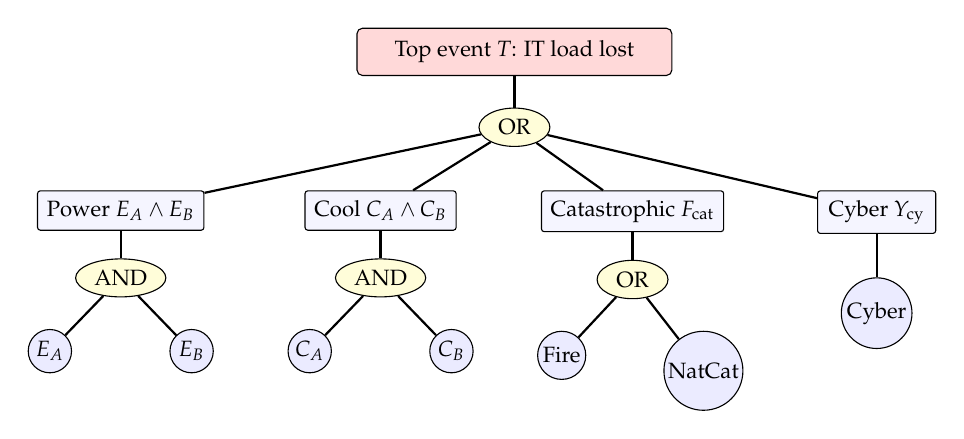
\begin{tikzpicture}[
   every node/.style={font=\footnotesize},
   top/.style={draw,rectangle,rounded corners=2pt,fill=red!15,minimum width=4cm,
               minimum height=0.6cm,align=center},
   gate/.style={draw,ellipse,fill=yellow!15,minimum width=0.9cm,minimum height=0.45cm,
                inner sep=2pt},
   bevt/.style={draw,circle,fill=blue!8,minimum size=0.55cm,inner sep=1pt,align=center},
   ievt/.style={draw,rectangle,rounded corners=1pt,fill=blue!4,minimum width=1.5cm,
                minimum height=0.5cm,align=center},
   ln/.style={thick}
]
% Top event
\node[top] (T) at (0,0) {Top event $T$: IT load lost};
\node[gate,below=0.4cm of T] (G0) {OR};
\draw[ln] (T) -- (G0);

% Four branches
\node[ievt,below=0.55cm of G0,xshift=-5.0cm] (EA) {Power $E_A\wedge E_B$};
\node[ievt,below=0.55cm of G0,xshift=-1.7cm] (CA) {Cool $C_A\wedge C_B$};
\node[ievt,below=0.55cm of G0,xshift= 1.5cm] (FC) {Catastrophic $F_{\mathrm{cat}}$};
\node[ievt,below=0.55cm of G0,xshift= 4.6cm] (CY) {Cyber $Y_{\mathrm{cy}}$};
\draw[ln] (G0) -- (EA);
\draw[ln] (G0) -- (CA);
\draw[ln] (G0) -- (FC);
\draw[ln] (G0) -- (CY);

% Power AND
\node[gate,below=0.35cm of EA] (G1) {AND};
\draw[ln] (EA) -- (G1);
\node[bevt,below=0.4cm of G1,xshift=-0.9cm] (EAfail) {$E_A$};
\node[bevt,below=0.4cm of G1,xshift= 0.9cm] (EBfail) {$E_B$};
\draw[ln] (G1) -- (EAfail);
\draw[ln] (G1) -- (EBfail);

% Cooling AND
\node[gate,below=0.35cm of CA] (G2) {AND};
\draw[ln] (CA) -- (G2);
\node[bevt,below=0.4cm of G2,xshift=-0.9cm] (CAfail) {$C_A$};
\node[bevt,below=0.4cm of G2,xshift= 0.9cm] (CBfail) {$C_B$};
\draw[ln] (G2) -- (CAfail);
\draw[ln] (G2) -- (CBfail);

% Catastrophic OR
\node[gate,below=0.35cm of FC] (G3) {OR};
\draw[ln] (FC) -- (G3);
\node[bevt,below=0.4cm of G3,xshift=-0.9cm] (FB) {Fire};
\node[bevt,below=0.4cm of G3,xshift= 0.9cm] (NC) {NatCat};
\draw[ln] (G3) -- (FB);
\draw[ln] (G3) -- (NC);

% Cyber leaf
\node[bevt,below=0.55cm of CY] (CYb) {Cyber};
\draw[ln] (CY) -- (CYb);

\end{tikzpicture}%
\end{document}
